\chapter{Evaluation}
\label{lab:eval}

In the previous chapter, the implementation characteristics of an actor-based Web framework were observed from the view of a developer (see chapter \ref{sec:impl}). While these aspects are important during the development of an application, once the application is publicly accessible, performance is a paramount factor. This chapter documents tests conducted with respect to performance criteria defined in chapter \ref{lab:technical} -- for example request frequency and response time (see section \ref{lab:frequency}) -- and aims to define use-cases for synchronous and asynchronous application structure in the context of Web frameworks.

\section{Prerequisites}

Modern Web server performance can be defined by the system's behaviour when processing a high number of simultaneous requests. Ideally, the response time for each request should be as low as possible and should not increase significantly with the number of simultaneous requests. 

To test the behaviour of thread-based applications side by side to event-based applications, tests should preferably be conducted under very similar conditions, the only major difference being asynchronous processing. Since in section \label{lab:lang} the \textit{Play!} framework was identified  as a feasible choice for demonstrating asynchronous processing in Web frameworks, \textit{Play!} is also used in the following performance tests. To achieve comparable performance, the thread-based contender application should ideally also be run on the \textit{Java} virtual machine (JVM). This leaves numerous choices due to the high number of \textit{Java}-based Web frameworks. The first choice was the \textit{Grails}\footnote{\url{https://grails.org/}} framework, which is based on \textit{Groovy}\footnote{http://groovy.codehaus.org/} language. Since \textit{Groovy} -- like \textit{Scala} -- is also an extension language to \textit{Java} and can be run on the \textit{Java} VM, it seemed like a good choice to compare to \textit{Play!}. However, \textit{Grails} proved to have a much larger memory footprint compared to \textit{Play!} and even exceeded the 512MB memory limit on the server container (see below). This imbalance ruled out \textit{Grails} as a fitting contender. The \textit{Spring MVC}\footnote{\url{http://spring.io/}} framework was the next Web framework taken into consideration. \textit{Spring MVC} is regarded as a similar solution compared to \textit{Play!}, especially when it comes to application structure and runtime behaviour \cite[p. 109]{Scala}. As its name implies, \textit{Spring MVC} features a comparable MVC (Model-View-Controller) structure; however, \textit{Spring MVC} does not include its own Web server, but can be executed on a number of different servers. In order to provide similar capabilities as \textit{Play!}'s integrated \textit{Netty} server (see section \ref{lab:play}, \textit{Performance}), \textit{Jetty}\footnote{\url{http://www.eclipse.org/jetty/}} was used as a Web server for the \textit{Spring MVC} application.

Obviously, to achieve neutral performance measurements, the two applications must be run on identical, yet independent systems. This, as well as the desire to simulate conditions also present in production setups, led to the decision to conduct the performance tests on virtual servers hosted by a \textit{cloud PaaS}\footnote{Platform as a Service. A computing platform provided by a third-party company using large-scale computing and networking systems.}. Due to the simplicity of deployment and replication, \textit{Heroku}\footnote{\url{http://www.heroku.com}} was the platform of choice. On \textit{Heroku}, various application technologies -- including \textit{Java} -- can be deployed and run within isolated containers in a controlled, reproducible fashion. The containers used for testing both are equipped with an \textit{Intel Xeon X5550} quad-core processor clocked at 2.67GHz and can address 512MB of memory.

Both applications were set up using their default configuration and using the \textit{Java} 7 platform. Tests were implemented as controller actions within the MVC environment and were triggered using HTTP requests to certain URLs, exactly as connecting via a website or HTTP interface would. Details on the individual tests are available in section \ref{lab:testing}. To simulate the response of the servers to large client demand, a single personal computer does not suffice. Manual testing, for instance with a browser, can only create several requests per second and even automated testing with tools like \textit{JMeter}\footnote{\url{http://jmeter.apache.org/}} may not produce desirable results due to limited bandwidth of a standard internet connections. Thus, a specialised online service that focusses on the simulation of large client loads under realistic conditions was used for testing; \textit{loader.io}\footnote{\url{https://loader.io/}} offers multiple options of load testing and the free plan supports up to 10000 concurrent connections per test.

\section{Testing} 
\label{lab:testing}
The first test conducted was a benchmark test to ensure that both systems perform equally in terms of raw computing power. To get an impression of processing speed, the time to complete an arithmetic integer operation can be measured. Initially, the recursive calculation of a certain number in the \textit{Fibonacci}\footnote{\textit{Fibonacci} numbers are produced by adding up the previous two numbers of the series, starting with 0 and 1.} series was chosen as a suitable calculation. However, the tests produced very different results between the \textit{Scala} and \textit{Java} applications. This is due to the fact that the \textit{Scala} compiler uses a technique called \textit{tail recursion}, which simplifies certain recursive constructs \cite{Malone2008}. Thus, an iterative implementation of the \textit{Fibonacci} algorithm was employed with almost equal outcome: The calculation of the 100000th \textit{Fibonacci} number took the \textit{Spring MVC} application 342 milliseconds and the \textit{Play!} application 340 milliseconds on average during ten passes.

After ensuring that both systems work with equal computation speed, the actual load tests can be conducted. \textit{loader.io} offers a test type that gradually increases the request frequency over a set amount of time; in all tests listed here, request frequency was increased during a timeframe of 30 seconds, meaning that each test lasted 30 seconds and then stopped. By measuring the average response time for a certain request frequency, the behaviour of the servers can be characterised. \textit{loader.io} offers a Web-based graph that displays this behaviour for one test per server; however, to acquire the graphs used in this chapter, a dedicated script gathered the different datasets and merged them to graphs that display the data for both applications with equal scale.

There are two main test categories. The first observes the behaviour of the servers for ``on-system operations'', i.e. calculations that demand computation time directly on the server -- like for instance image processing. The second category observes ``off-system operations'' like Web requests, database queries or cache lookups. Both categories feature a number of tests with varying parameters to generate different benchmarks of the server behaviour. During all tests, parameters were chosen in a way that generated interesting and meaningful results, but without compromising server stability; load was limited to the maximum both servers could handle without crashing.

On-system tests simulated server load by calculating a certain \textit{Fibonacci} number for each request, thus blocking either the Web thread (in the \textit{Spring MVC} application) or an actor-based worker thread (in the \textit{Play!} application). The complexity of the calculation was increased with different step sizes (with the linear increase rate of the request frequency being constant) and the most interesting results were chosen for presentation in the following section. 

Off-system tests loaded the content of a website (namely \textit{http://www.google.com}, which was chosen because of its resilience) and tunnelled it through the server applications to the client. This \textit{proxy}\footnote{A proxy server is a system that transmits network requests back and forth between client and target. This has different uses, for instance increased anonymity.}-like behaviour simulates operations that happen outside of the server system and block only threads on purely thread-based applications, while not consuming threads in event- and actor-driven applications. Since an increase in website size did not make much difference for the tests, the website to load was constant and the request frequency increase was increased with each test. Again, the most notable results were chosen for presentation.

\section{Results}
\subsection*{On-system Tests}
The first test was set up using the relatively fast calculation of the 1000th \textit{Fibonacci} number. A single request of this kind took both applications on average 170 milliseconds to process. However, with increasing request frequency, the average response times of the two applications drift apart with the \textit{Play!} application achieving generally lower response times, the difference being about 1000 milliseconds at 5000 requests per second (see figure \ref{fig:test1}). However, when increasing the computation complexity by calculating the 5000th \textit{Fibonacci} number -- resulting in an average response time of 300 milliseconds per request -- the response time difference between the two applications decreases with \textit{Play!} still being faster, but only with a difference of about 500 milliseconds at 5000 requests per second (see figure \ref{fig:test2}). A further increase of the computation complexity to the 10000th and 50000th \textit{Fibonacci} number -- resulting in 300 and 400 milliseconds average response time per request, respectively -- shows that the response times of the two applications become more and more similar until being nearly identical for the 50000th \textit{Fibonacci} number (see figures \ref{fig:test3} and \ref{fig:test4}).

\begin{figure}
\centering\small
\setlength{\tabcolsep}{0mm}
  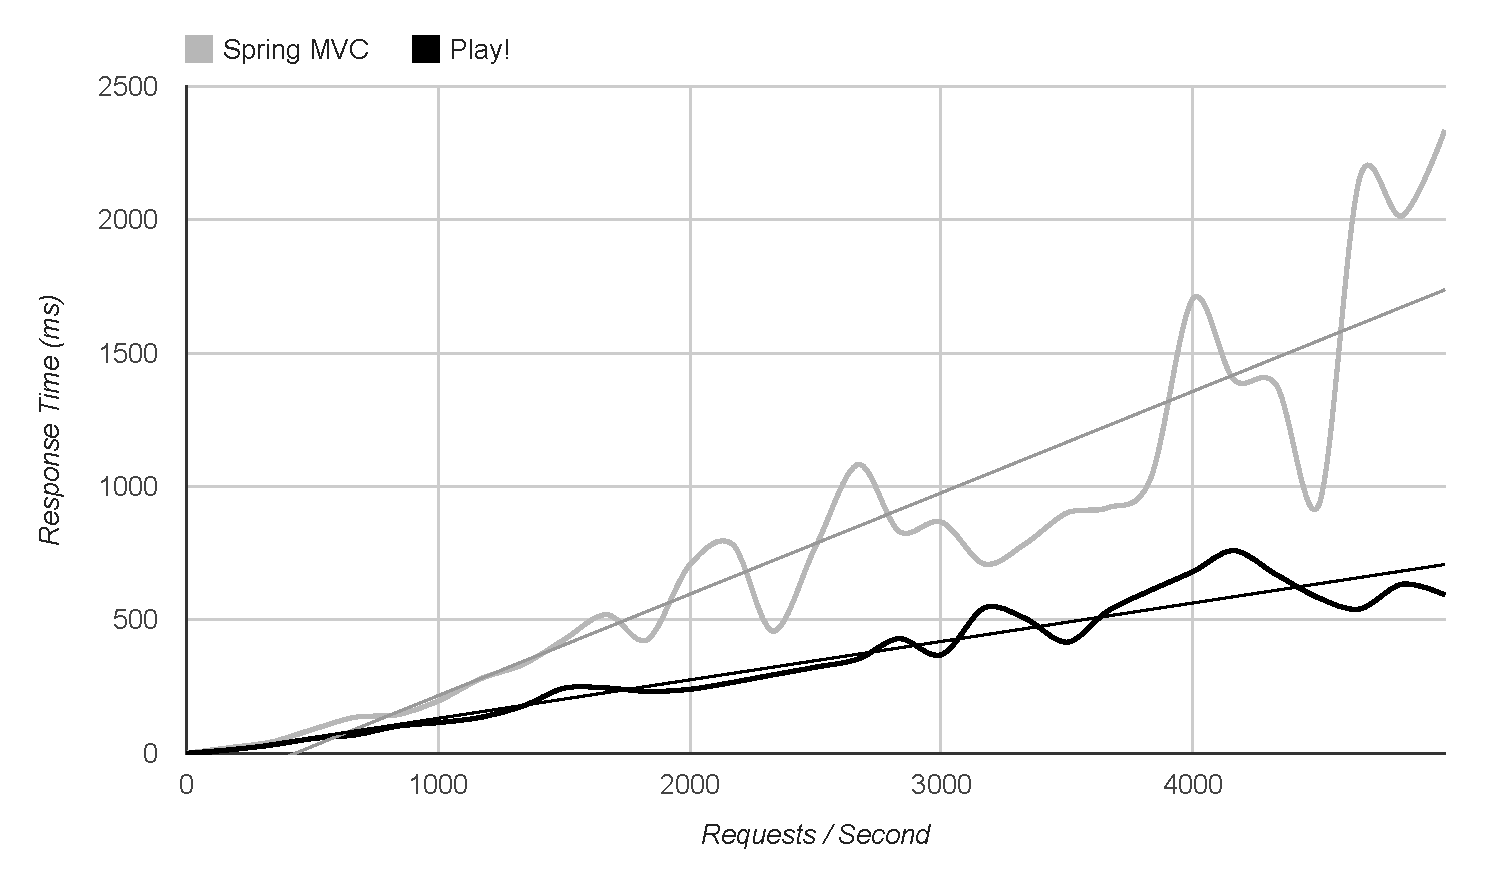
\includegraphics[width=.99\textwidth]{onsystem01test}
\caption{Iterative calculation of the 1000th \textit{Fibonacci} number. Request frequency is increased to 5000 within 30 seconds.
}
\label{fig:test1} 
\end{figure}

\begin{figure}
\centering\small
\setlength{\tabcolsep}{0mm}
  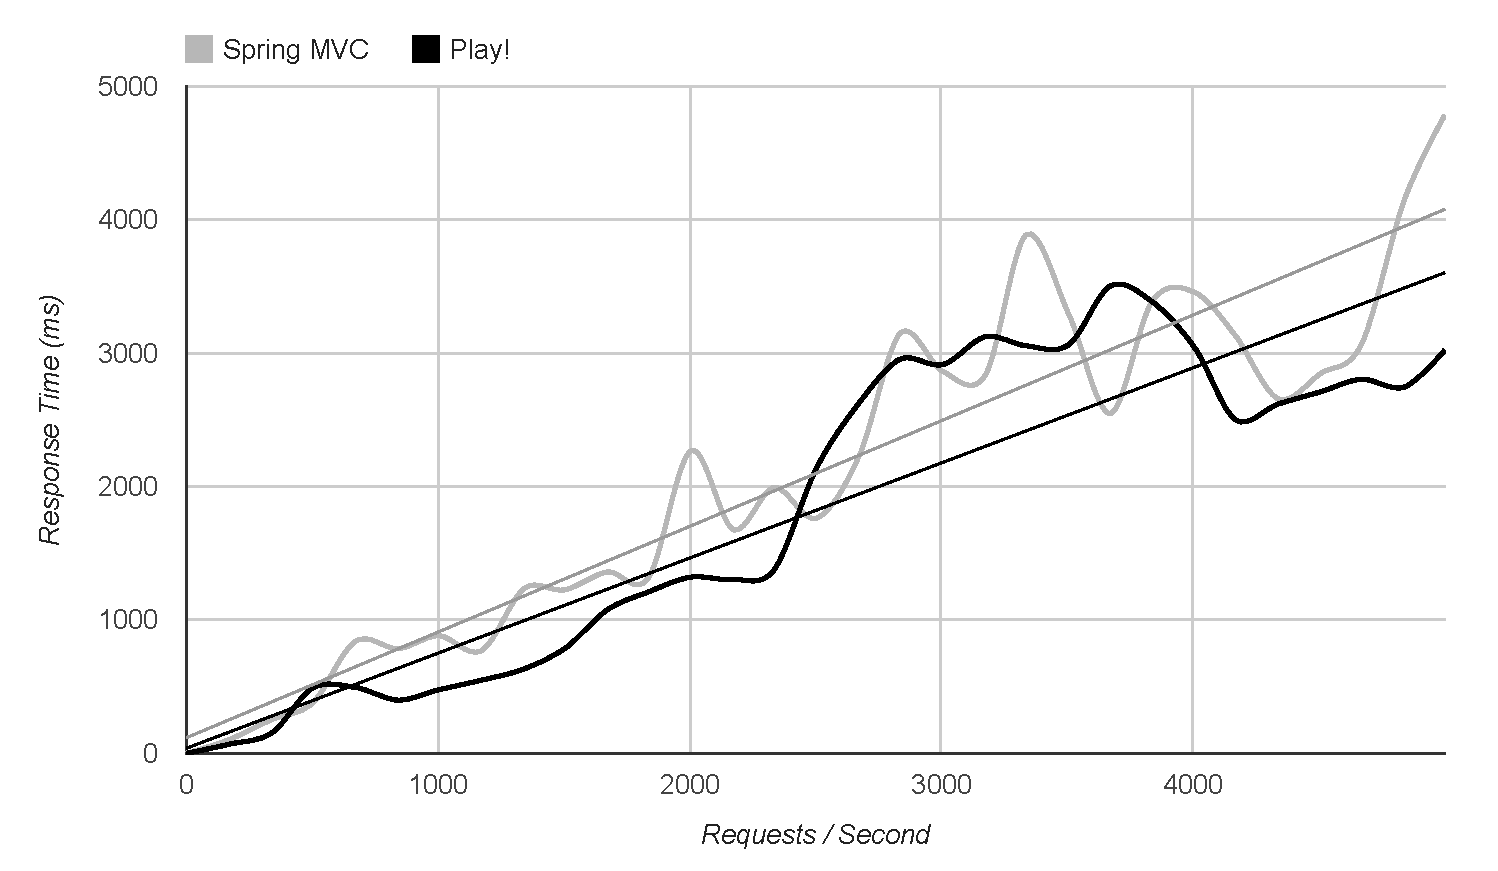
\includegraphics[width=.99\textwidth]{onsystem02test} 
\caption{Iterative calculation of the 5000th \textit{Fibonacci} number. Request frequency is increased to 5000 within 30 seconds.
}
\label{fig:test2} 
\end{figure}

\begin{figure}
\centering\small
\setlength{\tabcolsep}{0mm}
  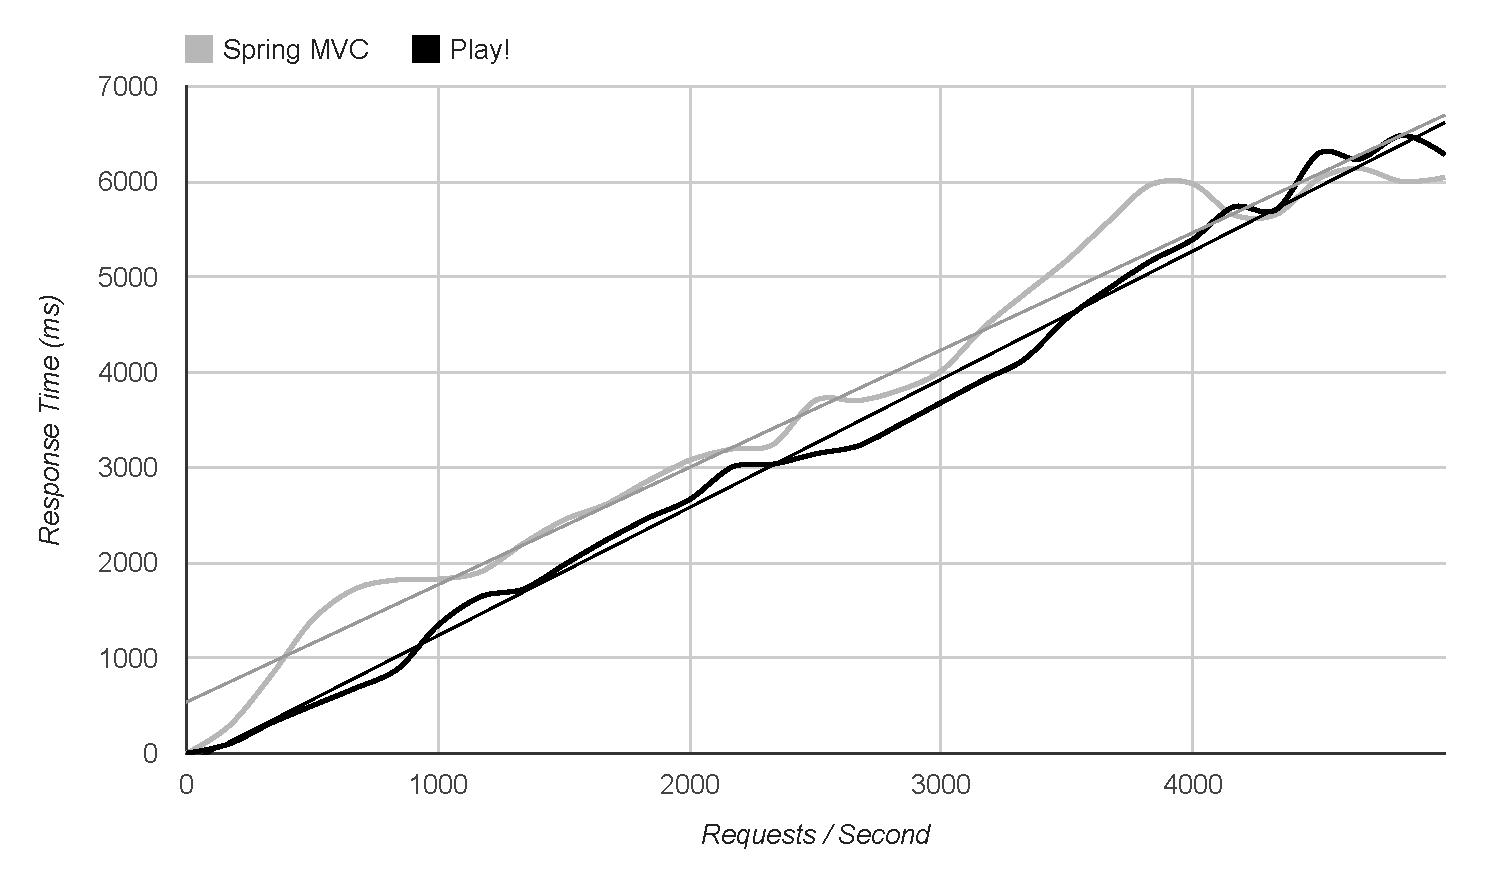
\includegraphics[width=.99\textwidth]{onsystem03test}
\caption{Iterative calculation of the 10000th \textit{Fibonacci} number. Request frequency is increased to 5000 within 30 seconds.
}
\label{fig:test3} 
\end{figure}

\begin{figure}
\centering\small
\setlength{\tabcolsep}{0mm}
  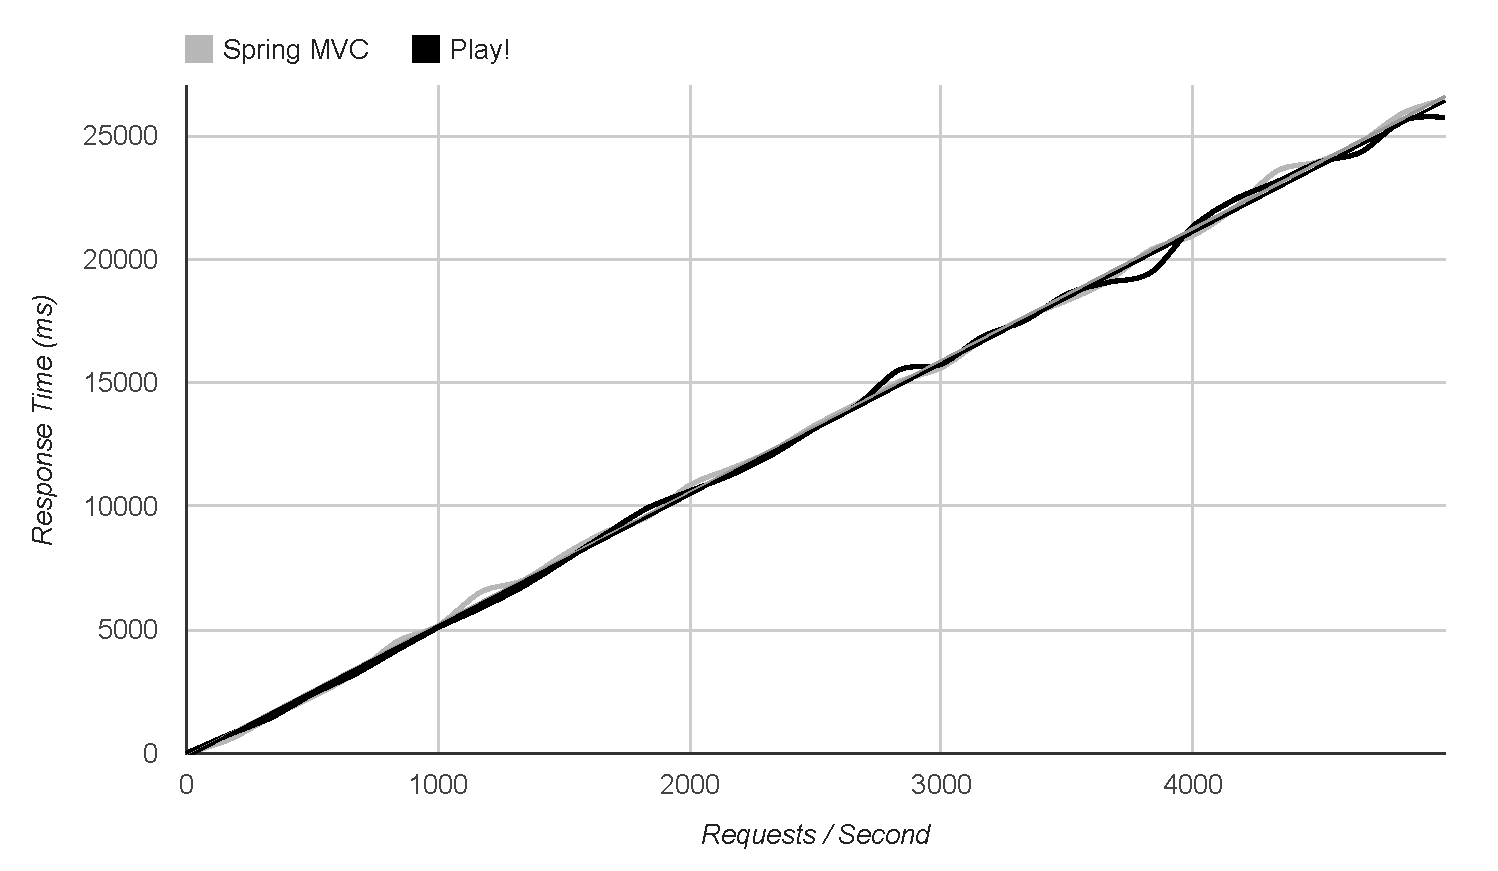
\includegraphics[width=.99\textwidth]{onsystem04test}
\caption{Iterative calculation of the 50000th \textit{Fibonacci} number. Request frequency is increased to 5000 within 30 seconds.
}
\label{fig:test4} 
\end{figure}

\subsection*{Off-system Tests}
As already mentioned in section \ref{lab:testing}, off-system tests were conducted by loading the content of the main page of \textit{Google}\footnote{\url{http://www.google.com}}, which, at the time of testing, contained 44 kilobytes of data and took about 170 milliseconds to load. Starting at a request frequency of 0 to 100 requests per second, the \textit{Play!} application outperforms the \textit{Spring MVC} application from about 30 requests per second and maintains low response times until the end of the test, while the response times of the \textit{Spring MVC} application continue to rise more steeply (see figure \ref{fig:test5}). Increasing the request frequency to 1000 exhibits even more pronounced results with the \textit{Play!} application being slower at the beginning, but from about 180 requests per second on maintaining a response time of about 800 milliseconds while the \textit{Spring MVC} application becoming ever slower until the difference accounts to about 2400 milliseconds at 1000 requests per second (see figure \ref{fig:test6}). During the third test of this category, request frequency is increased to 5000, obviously putting a lot of pressure on the applications. The response graph for this test looks very similar to the first graph of the on-system category (see figure \ref{fig:test1}) with response times of both applications increasing continuously at a high rate and the \textit{Play!} application being about 3800 milliseconds faster (see figure \ref{fig:test7}).


\begin{figure}
\centering\small
\setlength{\tabcolsep}{0mm}
  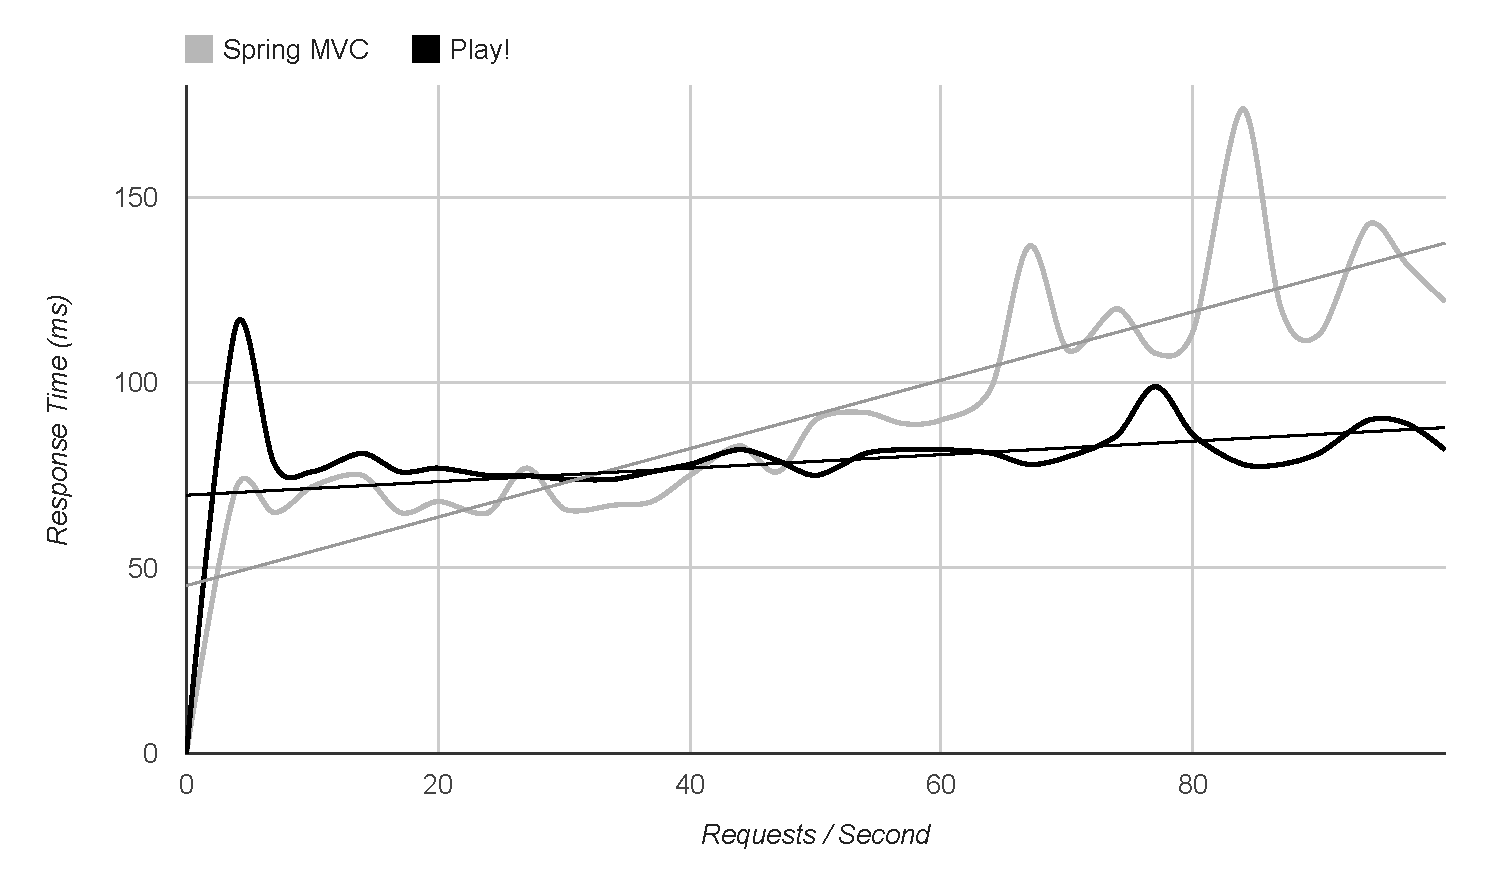
\includegraphics[width=.99\textwidth]{offsystem01test}
\caption{Loading and serving an off-system website. Request frequency is increased to 100 within 30 seconds.
}
\label{fig:test5} 
\end{figure}

\begin{figure}
\centering\small
\setlength{\tabcolsep}{0mm}
  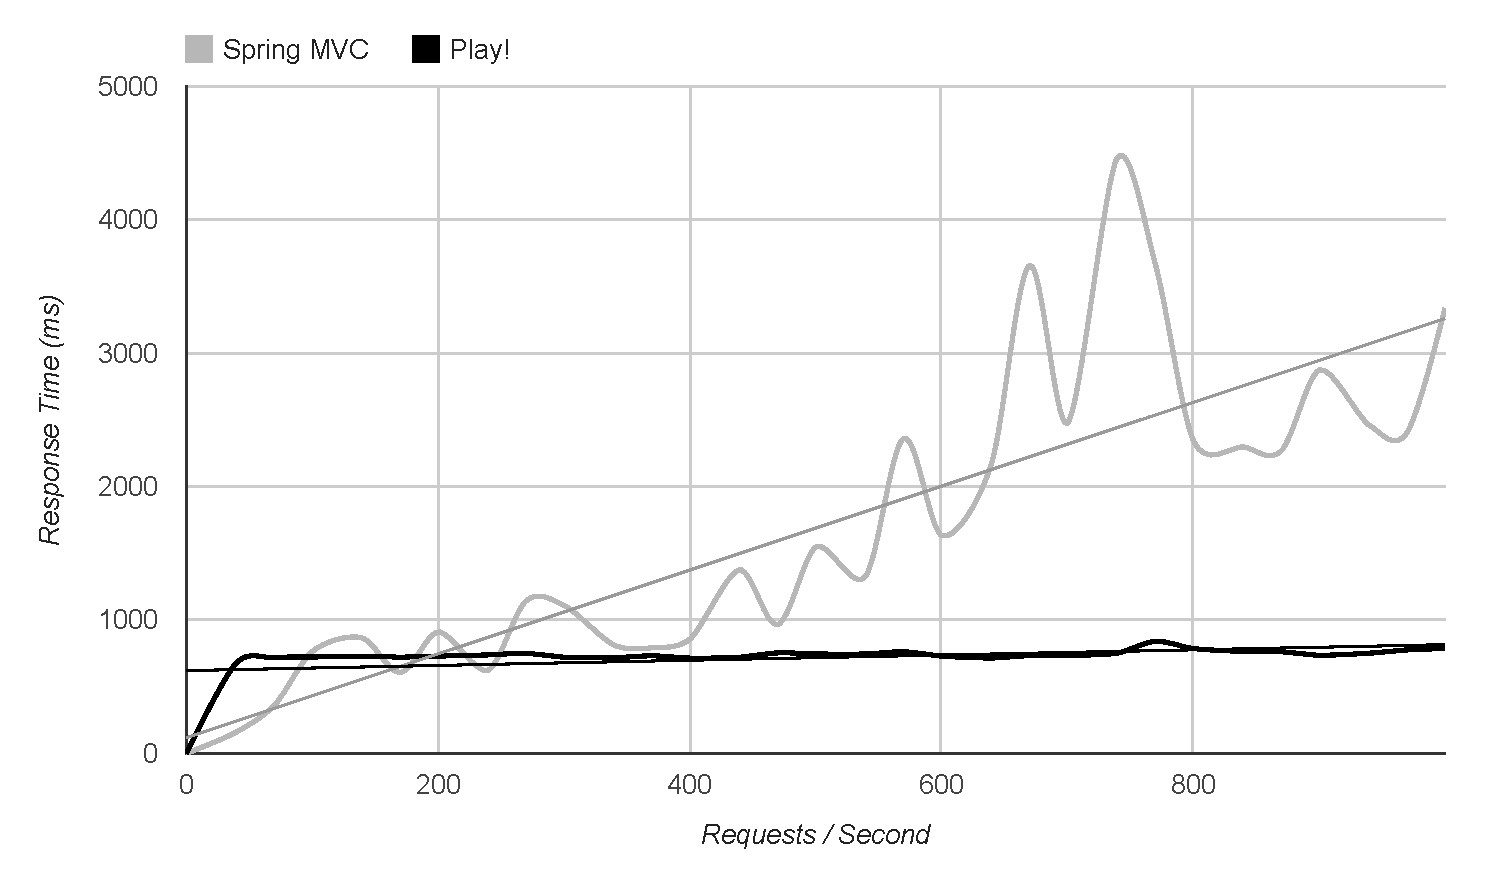
\includegraphics[width=.99\textwidth]{offsystem02test}
\caption{Loading and serving an off-system website. Request frequency is increased to 1000 within 30 seconds.
}
\label{fig:test6} 
\end{figure}

\begin{figure}
\centering\small
\setlength{\tabcolsep}{0mm}
  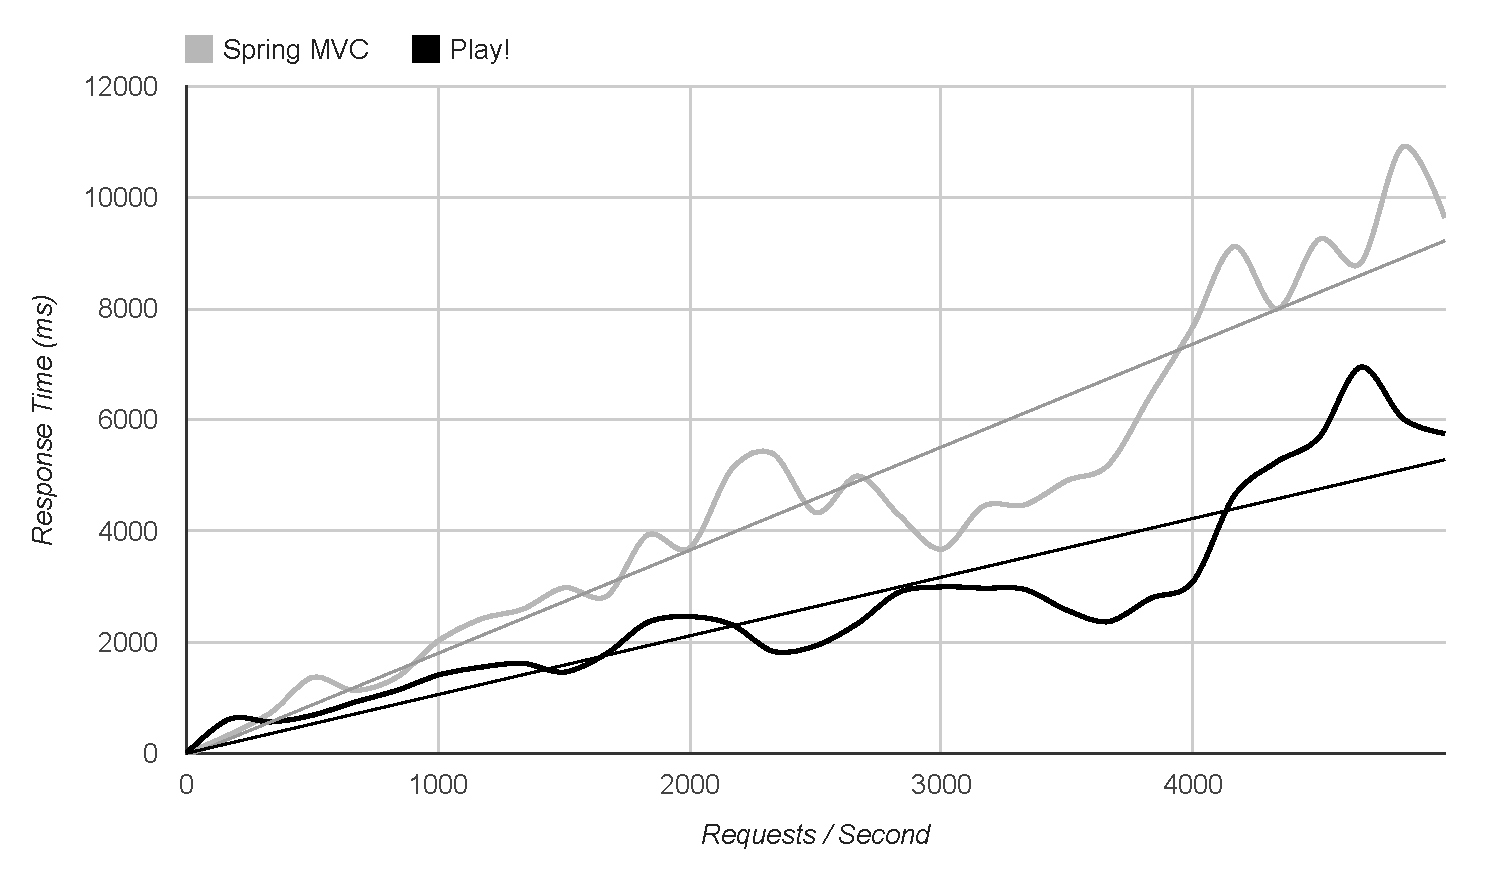
\includegraphics[width=.99\textwidth]{offsystem03test}
\caption{Loading and serving an off-system website. Request frequency is increased to 5000 within 30 seconds.
}
\label{fig:test7} 
\end{figure}

\section{Interpretation}
Looking at the tests, it is obvious that there is a significant difference between the on-system and off-system tests. In the on-system scenario, the performance difference between the blocking and the non-blocking application decreases with increasing server load while in the off-system scenario, the performance difference increases. Regarding the concurrency models detailed in section \ref{sec:concurrency}, this behaviour can be explained with the different resource usage on the servers. The context-switching overhead of the purely thread-based \textit{Spring MVC} application leads to a slower performance at a lower request frequency, while the actor-based \textit{Play!} application employs worker threads and reuses the same threads for network communication and request handling. However, with increasing computation complexity, the processing resources of both systems tend to be consumed wholly, which practically annihilates any advantage of lower context-switching overhead and worker threads; since both systems use identical hardware, both processors are saturated at the same point.

With off-system operations, on the other hand, the outcome is completely different. While the \textit{Play!} application achieves slower response times at the beginning due to the computational intensity of maintaining and orchestrating the actor system, it does not use up threads while waiting on the answer of the off-system Web server. Thus, up to a certain point, the \textit{Play!} application can maintain almost equal response times even with an increasing request frequency. The \textit{Spring MVC} application does not disengage the current thread during waiting for the response; this effectively blocks the current thread, raising the need to create or use another thread for the next incoming request. This puts more pressure on the operating system scheduler and creates contest-switching overhead. Moreover, since the processors used have four cores, only four threads can achieve physical concurrency at once; therefore, the \textit{Play!} application can use resources more efficiently by at all times doing active computations on all cores. However, when the request frequency exceeds the speed with which the \textit{Play!} application can handle communication with the off-system Web server, response times increase with actor queue size. This again creates a scenario in which the response time is directly proportional to the request frequency, much like with non-saturated on-system operations.












































